\documentclass{article}
\usepackage[utf8]{inputenc}
\usepackage{authblk}
\usepackage[russian,english]{babel}
\usepackage{amsmath}
\usepackage{amsfonts}
\usepackage{bm}
\usepackage{graphicx}
\usepackage{hyperref}
\usepackage{comment}
\usepackage{tikz}
\usetikzlibrary{positioning}
\usetikzlibrary{patterns}
\usepackage{pgfplots}
\usepackage{filecontents}
\usepackage{animate}
\usepackage{graphics}

\usepackage{subcaption}
\usepackage{caption}

\usepackage{tikz}
\usetikzlibrary{decorations.pathreplacing}

\title{\textbf{Methods of visualisation for flows with internal waves attractors}}
\author[1,A]{D.A Ryazanov}
\author[2,B]{S.A. Elistratov}
\author[3,C]{I.N. Sibgatullin}
\author[4,A]{M.V.~Kraposhin}

\affil[A]{Ivannikov Institute for System Programming of the RAS}
\affil[B]{Lomonosov Moscow State University}
\affil[C]{Shirshov Institute of Oceanology of Russian Academy of Sciences}
\affil[ ]{}
\affil[1]{ORCID: 0000-0001-9568-7121}
\affil[2]{ORCID: 0000-0002-7006-6879}
\affil[3]{ORCID: 0000-0003-2265-3259}
\affil[4]{ORCID: 0000-0001-5730-2702}

%Ivannikov Institute for System Programming of the RAS, Lomonosov Moscow State University, Shirshov Institute of Oceanology of Russian Academy of Sciences.

\date{}

\begin{document}

\maketitle

\underline{\textbf{Abstract}}

Application of different approaches to visualise hydrodynamic fields of internal waves is closely connected with the possibility of extracting important numerical characteristics of the flows. In this paper we describe methods of visualisation, which were shown to be very effective for illustration of the internal wave attractors both for laboratory experiments and numerical simulations. On the other hand, novel approaches for description of the wave flows with accumulation of energy are discussed. Methods of vortices identification show an interesting properties of the wave flows, and give an alternative for estimation of the width of wave beams. At the same time, the limitations of the applicability of the described methods depend on the resolution of the available data, which is especially important in the areas of the internal wave beams reflection.  

The article describes simulation of internal waves attractors in various statements.

\textbf{Keywords:} CFD, internal waves, inertial waves, post-processing, wave attractor

\section{Introduction}

Internal waves are may be the most common types of waves in oceans, since even the surface seems to be calm the deep-ocean waves are always present []. Oceanologists, biologists, ecologists, technicians, all have specific  interests in the study of internal waves. This phenomenon is responsible for the vertical mixing of the stratified fluids, the migration of living organisms, the redistribution of energy in the ocean, and the propagation of various kinds of impurities and pollution.

% Откуда пошли внутренние волны

The main condition for internal wave appearance is the density stratification of the fluid. 

One of the internal wave sources is the tidal effect produced by the orbital motion of the Moon. This global flow generates internal waves while interacting with the ocean bottom irregularities. The very special feature of the internal waves is the angle of their spreading and the law of reflection defined by the dispersion relation:

$$\frac{\omega}{N} = \sin(\theta),$$
where $\omega$ is forcing frequency determined by external impact on the fluid; 
$N$~-- buoyancy frequency.

% Пояснительная картинка с распространением
% Фокусировка внутренних волн

Due to these properties internal waves can be focused when after reflection from the oblique wall. As a consequence,  the internal wave wavelength reduces after reflection but its amplitude increases.

% Аттракторы внутренних волн
% картинка с резервуаром

In this case the great interest is the result of the multiple focusing. It can be obtained by the monochromatic excitation of the internal waves in the closed domain with the oblique boundaries, the simplest example of which is the rectangular trapezoid.

If the internal waves reflect in trapezoid vessel, focusing occurs continuously and their rays converge to closed trajectory. The simplest one is the rhomboid trajectory with four reflection points (Fig. \ref{fig:dominleft}).
%лучи выше

\begin{figure}[!ht]
    \centering
        \begin{tikzpicture}[scale=1.5, z={(-.707,-.5)}]
            \draw (0,4-0,0) -- (6,4-0,0) -- (4,4-4,0)--(0,4-4,0) --cycle;
            \draw (0,4-0,0)     -- (6,4-0,0)   -- (4,4-4,0)   -- (0,4-4,0)    -- cycle;
            \draw[style = dashed,red] (2.7,4-4,0)   -- (0,4-1.8,0) -- (2.2,4-0,0) -- (4.97,4-2.1,0)-- cycle;

            \draw[<->] (-0.1,4-0) --node[above,rotate=90] {$H$} (-0.1,4-4);
            \draw[<->] (0,4+0.1,0) --node[above,] {$L_2$ } (6,4+0.1,0);
            \draw[<->] (0,4-4.1,0) --node[below,] {$L_1$ } (4,4-4.1,0);

            \draw[thick,->] (4.95,4-4,0) -- (5.95,4-4,0) node[anchor=north east]{$x$};
            \draw[thick,->] (4.95,4-4,0) -- (4.95,4-3,0) node[anchor=north west]{$z$};
            \draw[thick,->] (5.5,4-2,0) -- (5.5,4-3,0) node[anchor=west]{$\vec{g}$};
        \end{tikzpicture}
    \caption{Scratch of the domain and attraction area}
    \label{fig:dominleft}
\end{figure}


% визуализация аттракторов внутренних волн предыдущие работы

For the first time this field was investigated by Leo Maas \cite{Maas1995} who studied the convergence of attractor rays to the trajectory depending on the geometry and internal waves reflection angle numerically via the ray-tracing method.


\section{Problem statement and solution methods}

For the stratified fluid dynamic simulation quasihydrodynamic equations were used \cite{ElizarBook}: 

 \begin{equation}
     \nabla \cdot \left (\vec U - \vec W \right ) = 0,
     \label{eq:cont}
 \end{equation}
 \begin{equation}
     \frac{\partial \vec U}{\partial t}  + \nabla \cdot \left ( (\vec U - \vec W)\otimes \vec U  \right )
     -
     \nabla \cdot \nu \left ( \nabla \vec U + (\nabla \vec U)^T \right ) - \nabla \cdot \left  (   \vec U \otimes \vec W \right ) 
      = - \frac{1}{\rho_m} \nabla \hat p + \vec F,
      \label{eq:mom}
 \end{equation}
     
 \begin{equation}
     \frac{\partial s}{\partial t} + \nabla \cdot \left ( (\vec U - \vec W)s \right )
     - \nabla \cdot \frac{\nu}{Sc} \left ( \nabla s \right )=0.
     \label{eq:tr}
 \end{equation}


Additional velocity:  $$\vec W = \tau \left ( \vec U \cdot \nabla \vec U + \frac{1}{\rho_m} \nabla \hat p - \vec F  \right ),$$\\

reduced pressure $\hat p = p - p_0$; restorative force: $\vec{F}=\beta \vec{g} \hat s$, where $\hat s = s(x, y, z, t) - s(x, y, z, 0).$

Geometrically the computational domain is the rectangular trapeze, on the left wall of which a wavemaker is situated. The letter one makes oscillations. 

Velocity boundary conditions on wavemaker depends on problem being solved.

Boundary conditions on static walls:

\begin{equation}\label{eq:qhd_walls}
        \vec{U} = 0, \,\,\, \frac{\partial \tilde p}{ \partial \vec{n}} = \rho_0 \vec n \cdot \left ( -\vec U_b \cdot \nabla \vec U + \vec F \right), \,\,\, \frac{\partial s}{ \partial \vec{n}} = 0.
\end{equation}

The initial conditions for a passive scalar are chosen so that the buoyancy frequency is equal to 1

\begin{equation}
    N(z) = \sqrt{- \frac{g}{\rho_m}\cdot\frac{d \rho(z)}{dz}} = 1,
\end{equation}

where $\rho(z) = \rho_m(1+\beta s)$  and $\beta$ -- coefficient of salinity contraction. 



Equations \ref{eq:cont}--\ref{eq:tr} solve by finite volume method and open source code OpenFOAM v2012 with QHDFoam solver \cite{QGDFOam}

\begin{figure}[b]
 \centering
 \begin{tikzpicture}[scale=1.88]
    \draw [decorate,decoration={brace,amplitude=10pt},xshift=-4pt,yshift=0pt] (-0.2,0.0) -- (-0.2,4.1) node[rotate=90,above] [black,midway,xshift=-0,yshift=10] { Wavemaker};
     \node[anchor=south west,inner sep=0] at (0,0) {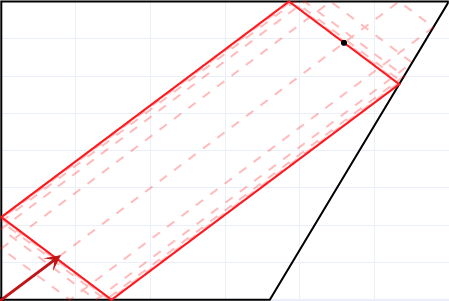
\includegraphics[width=0.95\textwidth]{Figs/Dom.png}};
     \draw[thick,<->] (-0.1,0) --node[above,rotate=90]{$H$} (-0.1,4.1);
     \draw[thick,<->] (0,-0.1) --node[below          ]{$L_2$} (3.8,-0.1);
     \draw[thick,<->] (0,4.2) --node[above          ]{$L_1$} (6.2,4.2);
     \draw [black, thick] (5.75,4.1) arc [start angle=180, end angle=270, radius=0.25cm];
 \end{tikzpicture}
 \caption{Principal scheme of the vessel}
 \label{fig:Domain}
\end{figure}



\section{Post-processing and data analysis}

All data was collected using native openFoam functionObjects and processed by python-scripts. Fields was visualised by open-source, multi-platform data analysis and visualization application paraview \cite{paraview}.

\subsection{2D statement}

As the calculation results, it is expected that internal waves will concentrate in the zone of attraction (Fig. \ref{fig:Domain}). In this case $H = 0.4 \; m$, $L_1=0.6 \; m$, $L_2 = 0.39 \; m$.

As boundary conditions on wavemaker:

\begin{equation}
    U_x = A\cdot cos\left(\frac{\pi \cdot z}{H}\right)\cdot \omega \cdot  sin(\omega_0 t),
    \label{eq:wmc}
\end{equation}
where $A = 0.003 \; m$, $\omega = 0.63 \; \frac{1}{s}$.

Dynamic of velocity fluids field over time can be spit in two smooth parts.

Part of attractor formation (Fig. \ref{fig:attr2dForm}). Internal waves reflect from slope wall and aim to attractor with increasing own aplitude.

\begin{figure}
    \centering
    \animategraphics[autoplay,loop,scale=0.3]{10}{Figs/2DAttractorForm/300x200a03w0623.0}{180}{200}
    \caption{Formation of attractor from $t=90\;s$ to $t=100\;s$}
    \label{fig:attr2dForm}
\end{figure}

Part of attractor destruction (Fig. \ref{fig:attr2dDests}). Gradually amplitude grows so much that the waves begin to overturn and generate child waves.

\begin{figure}
    \centering
    \animategraphics[autoplay,loop,scale=0.3]{10}{Figs/2DAttractorDest/300x200a03w0623.7}{160}{199}
    \caption{Destroyed attractor from $t=3580\;s$ to $t=3600\;s$}
    \label{fig:attr2dDests}
\end{figure}

Visualisation of velocity field was provided by paraview software \cite{paraview}. The pictures \ref{fig:attr2dForm} and \ref{fig:attr2dDests} show horizontal component.

As the one of main method of analysis is time-frequency diagram which shown dynamic of spectrum (Fig. \ref{fig:tfd}). at the beginning of motion fluid has one clear frequency, but then attractor destruction leads to the generation of secondary waves and contamination of the spectrum. 

\begin{figure}
    \centering
    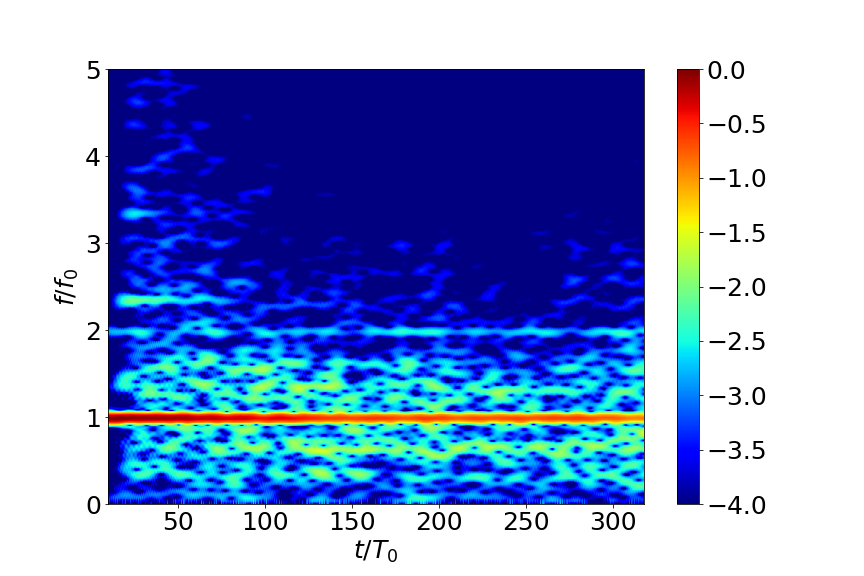
\includegraphics[scale=0.4]{Figs/TFD_pos34693_nperseg400_to0T.png}
    \caption{Time-frequency diagram of attractor destruction, $T_0$ -- period of wawemaker, $f_0$ -- freaquncy of wavemaker. ???}
    \label{fig:tfd}
\end{figure}

\subsection{Sedimentation}

One of the important problems is a simulation of low inertial particles sedimentation. Distribution of density in  the reservoir is linear from $1040\;\frac{kg}{m^3}$ to $1080\;\frac{kg}{m^3}$, at the center of the reservoir puts spherical particles with density $\rho_p = 1080;\frac{kg}{m^3}$ and diameter $d=0.001 \; m$.  Number of particles is 301 over horizontal middle line (Fig. \ref{fig:domainup}). Particles are carried away by the flow, but do not affect it and one another.

\begin{figure}[!ht]
    \centering
    \begin{tikzpicture}[scale=1.92, z={(-.707,-.5)}]
    \draw (3.6,0,0) -- (0,0,0) -- (0,4,0)--(6,4,0)--(3.6,0,0);
    %\draw (3.6,0,0) -- (3.6,0,-1) -- (6,4,-1) -- (6,4,0) -- cycle;
    %\draw (6,4,0) -- (0,4,0) -- (0,4,-1) -- (6,4,-1);
     \node[anchor=south west,inner sep=0] at (0,0) {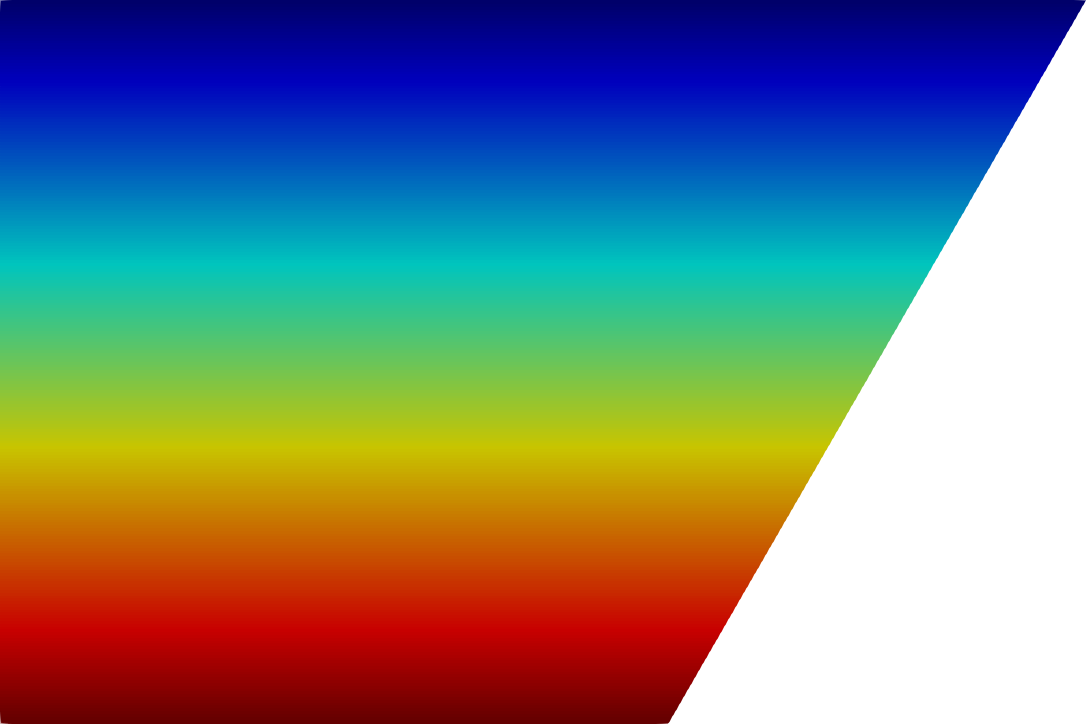
\includegraphics[width=0.95\textwidth]{Figs/Temp.png}};
    \draw (-0.5,2,0) node{};
    \draw (4.1,-.2,-1.5) node{};
    \draw [white] (3,3.8,0) node{$\rho_l = 1040$};
    \draw (1.8,2.1) node{$\rho_p = 1080$};
    \draw (2.9,2.1) node{$\rho_l = 1060$};
    \draw (2,0.2,0) node{$\rho_l = 1080$};
    \draw[<->] (-0.1,0) --node[above,rotate=90] {$H$} (-0.1,4);
    \draw[<->] (0,4.1,0) --node[above,] {$L_1$} (6,4.1,0);
    \draw[<->] (0,-0.1,0) --node[below,] {$L_2$} (3.7,-0.1,0);
    \draw [white, thick] (5.5,4) arc [start angle=180, end angle=240, radius=0.5cm]
        node [left] {$\alpha$};
    \draw[thick,->] (5.5,1,0) -- (6.5,1,0) node[anchor=north east]{$x$};
    \draw[thick,->] (5.5,1,0) -- (5.5,2,0) node[anchor=north west]{$z$};
    \draw[thick,->] (0,0,0) -- (2.5,1.6,0) ;
    \draw[thick,dotted] (0,2,0)--(4.8,2,0);
    \draw [black, thick] (0.42,0.28) arc [start angle=30, end angle=90, radius=0.5cm] node [above right] {$\theta$};
    
    \end{tikzpicture}
    \caption{Initial distribution of density. $\rho_l$ -- density of liquid, $\rho_l$ -- density of particles, $\theta = \arcsin \frac{\omega}{N}$, where $\omega$ is frequency of wavemaker and $N$ is the buoyancy frequency.}
    \label{fig:domainup}
\end{figure}

The simulation is of interest for two reasons: sedimentation process before particles touch the bottom and distribution process after sedimentation. Numerical experiment was carried out in two different statements for wavemaker conditions (\ref{eq:wmc}) with $A_1=0.05e^{-2}\;m$ -- regime of stable attractor without destruction and child waves and $A_2=0.003\;m$ turbulent attractor of internal waves from previous subsection. 

\begin{figure}
\centering
    \begin{minipage}{0.45\textwidth}
        \centering
    \animategraphics[autoplay,loop,scale=0.12]{10}{Figs/2DSedTurbBegin/AnimationRho1080C0r01mmslip.0}{000}{159}
        \subcaption[fir]{Sedimentation from $t=0\,s$ to $t=80\,s$}
        \label{fig:turbSed2Da}
    \end{minipage}
    \begin{minipage}{0.45\textwidth}
        \centering
    \animategraphics[autoplay,loop,scale=0.125]{10}{Figs/2DSedTurbEnd/AnimationRho1080C0r01mmslip.7}{013}{052}
        \subcaption[sec]{Redistribution from $t=3590 \,s$ to $t=3600$}
        \label{fig:turbSed2Db}
    \end{minipage}
    \caption{Sedimentation in reservoir with turbulent regime of internal waves attractor}
\end{figure}

Numerical experiment shown that particles slow fall and redistribute (Fig. \ref{fig:turbSed2Da}). Fallen particles concentrate about two attraction center at the bottom (Fig. \ref{fig:turbSed2Db}).

\subsection{3D local wavemaker}


\subsection{Vortices visualisation}

Vortices visualisation is a new way to visualize turbulent motions structure. For this purpose we use different methods.

The simplest attempt is to consider vorticity \cite{vortex}: $$\omega=\textrm{rot}\,\vec{v}$$
It is quick and simple method that however can yield false-positive identification. For instance, Couette flow will be identified as homogeneous vortex since its curl is constant over the domain.

Another method is so-called $\Delta$-method \cite{vortex}. Let us consider eigenvalue problem for velocity gradient tensor $A=\nabla\otimes  \vec v$:

% \begin{equation}
%  A:= \nabla\otimes  \vec v =
% \begin{pmatrix}
%  \frac{\partial v_x}{\partial x}  & \frac{\partial v_x}{\partial y} \\ \frac{\partial v_y}{\partial x} & \frac{\partial v_y}{\partial y} 
% \end{pmatrix}
% \end{equation}

\begin{equation}
  \text{det} \, A -\lambda \mathbb E=0
\end{equation}  

In 3D we have the following characterstical equation: $$\lambda^3+P\lambda^2+Q\lambda+R,$$ \noindent which discriminant is $D=-108\left( \frac{Q^2}{4} +\frac{P^3}{27}\right)$. 


Let $$\Delta=\left(\frac{Q}{2}\right)^2 +\left(\frac{P}{3}\right)^3$$

$ \Delta > 0 $ <=> $D<0$ means the presence of two complex-conjugated roots, i.e. current tubes is spiral-like shaped.

The problem arises in 2-dimensional problem, where the equation has less order:
$$\lambda^2+P\lambda+Q=0,$$

discriminant $D=P^2-4Q$. Thus in 2D we will consider $-D\equiv 4Q-P^2$ as $\Delta$.

This method requires more computational resources. It can be improved using $Q$-method \cite{vortex}\cite{Hussain}. Let's define:

\begin{equation}
 S=\frac{1}{2}\left(A +A\,^T \right) ,\quad \Omega=\frac{1}{2} \left( A - A\,^T\right) 
  \label{NSdim}
\end{equation}
Then
\begin{equation}
  Q=\frac{1}{2} \left( ||\Omega||^2_F-||S||^2_F \right) 
 \end{equation}

The vortex regions are those with $Q>0$. It is harder condition then that for the $\Delta$, so $Q$-identified vortex regions a priori contain in $\Delta$-identified ones.

Let's calculate eigenvalues of $A$. For the vortex presence it's necessary for two complex-conjugation values to exist. Their imaginary parts $\pm\lambda_{ci}$ that can be considered as the identification method itself \cite{vortex}.

If we consider eigenvalues of $S^2+\Omega^2$~matrix, we obtain $\lambda_2$-method. They cannot be complex, so let's sort them in descending order and consider the second one as a criterion \cite{vortex,Hussain}.

The most modern method is Luitex-method \cite{vortex}.

Let $\vec r \longleftrightarrow \lambda_r$~-- eigenvector corresponding to real eigenvalue $\lambda_r, ||\vec r||=1$. Then Luitex-vector is introduced as that with the direction of $\vec r$ and value
 $$R=(\vec \omega,\vec r)-\sqrt{(\vec \omega,\vec r)^2-4\lambda_{ci}^2},$$\noindent where $\vec \omega$ is vorticity. Wherein it's supposed that $(\vec \omega,\vec r)>0$.
 
 In 2-dimensional problem Luitex-vector must be re-defined. Obviously, vorticity is orthogonal to the domain plane as well as $\vec r$. Hence we concider only value
 
 $$R=|\omega|- \sqrt{\omega^2-4\lambda_{ci}^2},$$\noindent where $\omega=\frac{\partial v_y}{\partial v_x}-\frac{\partial v_x}{\partial v_y}$~-- two-dimensional vorticity.

\section{Conclusions}



\section{Acknowledgments}



The work will done with the support of Russian Scientific Fund, grant RSF~19-11-00169.
Authors thank T.G. Elizarova.

\bibliographystyle{ugost2008}
\bibliography{rpz}

\end{document}
